% Supplementary Material for the IEEE/ACM TCBB submission (ieee-article.tex).
% TCBB requires appendices and supplementary content to be uploaded as a
% separate file. Section, figure, table, and algorithm numbers carry an "S"
% prefix; the main text refers to them by these fixed numbers.

\documentclass[10pt,journal,compsoc]{IEEEtran}

\ifCLASSOPTIONcompsoc
  \usepackage[nocompress]{cite}
\else
  \usepackage{cite}
\fi

\usepackage{graphicx}
\usepackage{array}
\usepackage{booktabs}
\usepackage{amsmath,amssymb,amsfonts}
\usepackage{textcomp}
\usepackage{xcolor}
\usepackage[ruled,linesnumbered]{algorithm2e}
\usepackage{hyperref}

\renewcommand{\thesection}{S\arabic{section}}
\renewcommand{\thefigure}{S\arabic{figure}}
\renewcommand{\thetable}{S\arabic{table}}
\renewcommand{\theequation}{S\arabic{equation}}
\renewcommand{\thealgocf}{S\arabic{algocf}}

\begin{document}

\title{Supplementary Material for\\ ``Benchmarking Single-Cell Marker-State Forecasting Under Independent and Coupled Cell Pairings''}

\author{Victor~Ikenna~Kanu,
        Ihunanya~Udodiri~Ajakwe,
        Josiah~Ayoola~Isong,
        Simeon~Okechukwu~Ajakwe,
        and~Dong-Seong~Kim}

\markboth{IEEE/ACM Transactions on Computational Biology and Bioinformatics --- Supplementary Material}%
{Kanu \MakeLowercase{\textit{et al.}}: Forecasting Under Independent and Coupled Pairings}

\maketitle

\section{Datasets and Marker Programs}
\label{sup:data}

\subsection{Neural (dopaminergic) lineage}
The neural data are drawn from the population-scale induced-pluripotent-stem-cell (iPSC) to dopaminergic-neuron differentiation resource of~\cite{jerber2021population}, restricted to untreated control samples (treatment $=$ \texttt{NONE}) so that the trajectory reflects unperturbed differentiation. The raw series comprises $205{,}416$ cells across two treatment conditions; after restricting to untreated controls and standard quality control, $161{,}584$ cells are retained across three experimental stages: day~11 (D11, $50{,}661$ cells), day~30 (D30, $50{,}169$ cells), and day~52 (D52, $60{,}754$ cells). These stages span the transition from residual pluripotency through neural progenitor commitment to dopaminergic maturation.

\subsection{Cardiac (cardiomyocyte) lineage}
As an independent cross-lineage replication, the iPSC$\rightarrow$cardiomyocyte differentiation time-course of~\cite{elorbany2022single} (GEO accession \texttt{GSE175634}) is processed directly from raw counts using the identical pipeline. The deposited series contains $230{,}786$ cells profiled across seven timepoints (days 0, 1, 3, 5, 7, 11, 15) from more than twelve donor lines under a single directed protocol, with no treatment confound; annotation recovers the expected progression from iPSC through mesoderm and progenitor states to cardiomyocyte. The three-stage forecasting task uses day~0, day~5, and day~11 (early iPSC, mid-transition, committed cardiomyocyte; $41{,}330$, $19{,}508$, and $39{,}342$ cells respectively). These stages are chosen deliberately: they span the informative portion of the trajectory while avoiding the post-day-7 plateau, over which the differentiation score is near-constant and would contribute little dynamical signal. Before any modeling, the expected developmental biology was confirmed to be recovered under the present state construction: the pluripotency program extinguishes monotonically across the three stages (median $P$: $0.86\!\rightarrow\!0.15\!\rightarrow\!0.00$) and the cardiomyocyte program activates (median $D$: $0.00\!\rightarrow\!0.19\!\rightarrow\!0.22$).

\subsection{Marker panels}
For the neural data, $\mathcal{G}_P=\{\mathrm{POU5F1,\,NANOG,\,SOX2,\,UTF1,\,TDGF1}\}$ collects canonical pluripotency transcription factors, and $\mathcal{G}_D=\{\mathrm{TH,\,DDC,\,SLC6A3,\,DRD2,\,LMX1A,\,FOXA2}\}$ collects dopaminergic-identity and maturation genes spanning dopamine synthesis (\textrm{TH, DDC}), transport (\textrm{SLC6A3}), receptor (\textrm{DRD2}), and floor-plate fate (\textrm{LMX1A, FOXA2}). For the cardiac data the panels are lineage-appropriate analogues, a broadened pluripotency panel and a cardiomyocyte-identity panel:
\begin{align*}
\mathcal{G}_P^{\mathrm{card}}=\{&\mathrm{POU5F1,\,NANOG,\,SOX2,\,LIN28A,}\\
&\mathrm{DPPA4,\,UTF1,\,TDGF1}\},\\
\mathcal{G}_D^{\mathrm{card}}=\{&\mathrm{TNNT2,\,MYH6,\,MYH7,\,ACTC1,\,NPPA,}\\
&\mathrm{MYL7,\,TNNI1,\,TNNI3,\,RYR2,\,NKX2\text{-}5,}\\
&\mathrm{GATA4,\,TBX5,\,MYL2}\}.
\end{align*}
The cardiac differentiation panel spans sarcomeric structure (\textrm{TNNT2, MYH6/7, ACTC1, MYL2/7, TNNI1/3}), calcium handling (\textrm{RYR2}), natriuretic signalling (\textrm{NPPA}), and cardiac transcription factors (\textrm{NKX2-5, GATA4, TBX5}). All base-panel genes were present in their respective datasets with no missing markers. The dopaminergic panel is not transferred onto the cardiac data; doing so would conflate a lineage mismatch with the forecasting question under study.

\subsection{Normalization}
Raw counts are library-size normalized to $10{,}000$ counts per cell (CP10K) and log-transformed. For the neural data this uses Scanpy \texttt{normalize\_total}+\texttt{log1p}; for the cardiac data the identical transform is applied during a single streaming pass over the counts matrix, avoiding loading the full $230{,}786\times 38{,}943$ array. The qualitative stage-wise trends were verified to persist under unclipped scoring.

\section{Per-Seed Pseudo-Trajectory Construction}
\label{sup:alg}

Algorithm~\ref{alg:traj_norm} formalizes the pseudo-trajectory construction together with the leakage-safe normalization, written as the per-seed procedure actually executed: trajectory sampling, training-only split, training-bounds estimation, and normalization are all driven by a seed that is varied across runs.

\begin{algorithm}[!t]
\small
\caption{Per-Seed Pseudo-Trajectory Construction and Leakage-Safe Normalization}
\label{alg:traj_norm}
\textbf{Require:} scRNA-seq dataset $\mathcal{X}$ with stage labels $t\in\{t_0,t_1,t_2\}$, untreated/control filter $\phi(\cdot)$, marker panels $\mathcal{G}_P,\mathcal{G}_D$, trajectory count $N=200$, split sizes $(N_{\mathrm{tr}},N_{\mathrm{val}},N_{\mathrm{te}})=(140,30,30)$, seed $s$ \\
\textbf{Output:} Trajectories $\mathcal{T}=\{x^{(i)}\}_{i=1}^{N}$, split indices $(\mathcal{I}_{\mathrm{tr}},\mathcal{I}_{\mathrm{val}},\mathcal{I}_{\mathrm{te}})$, training bounds $\mathcal{B}$ \\
\BlankLine
\textbf{SetSeed}$(s)$ \tcp*{seed governs sampling \emph{and} split}
\tcp{Filter to untreated/control and partition by ground-truth stage}
$\mathcal{X}_0 \leftarrow \{x\in\mathcal{X}\;:\;\phi(x)=1\}$ \;
$\mathcal{X}_{t}\leftarrow \{x\in\mathcal{X}_0: \mathrm{stage}(x)=t\}$ \textbf{ for } $t\in\{t_0,t_1,t_2\}$ \;
\BlankLine
\tcp{Sample independent cells per stage and form ordered pseudo-trajectories}
\For{$i\leftarrow 1$ \KwTo $N$}{
    \For{$t \in \{t_0,t_1,t_2\}$}{
        $c_t \sim \mathcal{U}(\mathcal{X}_t)$ \tcp*{independent draw}
        $P^{\mathrm{raw}}_t\leftarrow \frac{1}{|\mathcal{G}_P|}\sum_{g\in\mathcal{G}_P}\log(1+\mathrm{expr}_{c_t}(g))$ \;
        $D^{\mathrm{raw}}_t\leftarrow \frac{1}{|\mathcal{G}_D|}\sum_{g\in\mathcal{G}_D}\log(1+\mathrm{expr}_{c_t}(g))$ \;
    }
    $x_{\mathrm{raw}}^{(i)}\leftarrow \big[(P^{\mathrm{raw}}_{t_0},D^{\mathrm{raw}}_{t_0}),(P^{\mathrm{raw}}_{t_1},D^{\mathrm{raw}}_{t_1}),(P^{\mathrm{raw}}_{t_2},D^{\mathrm{raw}}_{t_2})\big]$ \;
    $\mathcal{T}_{\mathrm{raw}}\leftarrow \mathcal{T}_{\mathrm{raw}}\cup\{x_{\mathrm{raw}}^{(i)}\}$ \;
}
\BlankLine
\tcp{Trajectory-level split, shared identically across all models}
$(\mathcal{I}_{\mathrm{tr}},\mathcal{I}_{\mathrm{val}},\mathcal{I}_{\mathrm{te}})\leftarrow \textbf{SplitIndices}(N,N_{\mathrm{tr}},N_{\mathrm{val}},N_{\mathrm{te}})$ \;
\BlankLine
\tcp{Min--max bounds from TRAINING trajectories only (prevents leakage)}
$\mathcal{S}_{\mathrm{tr}}\leftarrow \{(P^{\mathrm{raw}},D^{\mathrm{raw}})\in x_{\mathrm{raw}}^{(i)}: i\in \mathcal{I}_{\mathrm{tr}}\}$ \;
$P_{\min/\max}^{\mathrm{tr}}\leftarrow \min/\max \mathcal{S}_{\mathrm{tr}}(P^{\mathrm{raw}})$;\quad
$D_{\min/\max}^{\mathrm{tr}}\leftarrow \min/\max \mathcal{S}_{\mathrm{tr}}(D^{\mathrm{raw}})$ \;
$\mathcal{B}\leftarrow \{P_{\min}^{\mathrm{tr}},P_{\max}^{\mathrm{tr}},D_{\min}^{\mathrm{tr}},D_{\max}^{\mathrm{tr}}\}$ \;
\BlankLine
\tcp{Normalize all trajectories with training bounds and clip to $[0,1]$}
\For{$i\leftarrow 1$ \KwTo $N$}{
    \ForEach{$(P^{\mathrm{raw}},D^{\mathrm{raw}})\in x_{\mathrm{raw}}^{(i)}$}{
        $P\leftarrow \mathrm{clip}\!\big(\tfrac{P^{\mathrm{raw}}-P_{\min}^{\mathrm{tr}}}{P_{\max}^{\mathrm{tr}}-P_{\min}^{\mathrm{tr}}},0,1\big)$;\quad
        $D\leftarrow \mathrm{clip}\!\big(\tfrac{D^{\mathrm{raw}}-D_{\min}^{\mathrm{tr}}}{D_{\max}^{\mathrm{tr}}-D_{\min}^{\mathrm{tr}}},0,1\big)$ \;
        Replace $(P^{\mathrm{raw}},D^{\mathrm{raw}})$ with $(P,D)$ in $x^{(i)}$ \;
    }
    $\mathcal{T}\leftarrow \mathcal{T}\cup\{x^{(i)}\}$ \;
}
\BlankLine
\Return $(\mathcal{T},\mathcal{I}_{\mathrm{tr}},\mathcal{I}_{\mathrm{val}},\mathcal{I}_{\mathrm{te}},\mathcal{B})$
\end{algorithm}

\section{Model and Calibration Details}
\label{sup:models}

\subsection{Constant baselines}
Within each seed the constant training median is computed only from the training partition $\mathcal{I}_{\mathrm{tr}}$ ($140$ trajectories), separately for each target component, as $m_P=\mathrm{median}_{i\in\mathcal{I}_{\mathrm{tr}}}P^{(i)}_{t_2}$ and $m_D=\mathrm{median}_{i\in\mathcal{I}_{\mathrm{tr}}}D^{(i)}_{t_2}$, where the $P^{(i)}_{t_2},D^{(i)}_{t_2}$ are the late-stage states \emph{after} the training-bounds min--max normalization and clipping, i.e.\ on exactly the scale on which all other models are trained and scored. No further transformation or clipping is applied; because the training targets already lie in $[0,1]$, so do their medians. The same two numbers are returned for every validation and test trajectory of that seed, and the validation partition is not used. The constant training mean is defined identically with the mean in place of the median. Both constants are computed on exactly the per-seed trajectories and splits used by the other models; refitting Ridge on the regenerated data reproduces its stored per-seed MAE to within $10^{-16}$, confirming that the comparison is paired.

\subsection{Classical baselines}
Ridge regression ($\alpha=1.0$) is a linear map $\hat{s}_{t_2}=Wx+b$ with $W\in\mathbb{R}^{2\times4}$, $b\in\mathbb{R}^2$. In the multi-seed experiments the random forest is complexity-matched by tuning per seed with 3-fold cross-validation on the training partition only (300 trees; maximum depth $\in\{2,3,5,\text{unbounded}\}$; minimum samples per leaf $\in\{1,5,10\}$; MAE scoring). The single-seed leakage analysis (Sec.~\ref{sup:leakage}) reproduces the original fixed configuration (100 trees, maximum depth 10, minimum samples per split 5). An under-regularized fixed-depth forest appears modestly worse than the tuned forest, but this reflects overfitting of a high-capacity learner on a small task with no input--target dependence rather than any Transformer advantage; the regularized forest performs no better than the constant training mean, like the linear baseline.

\subsection{Transformer}
The encoder treats $[s_{t_0},s_{t_1}]$ as a length-two token sequence:
\begin{equation}
h_t = W_e s_t + b_e + \mathrm{PE}(t),\qquad
\hat{s}_{t_2} = \mathrm{MLP}\big(\mathrm{Enc}([h_{t_0},h_{t_1}])_{t_1}\big),
\end{equation}
with $W_e\in\mathbb{R}^{d_{\mathrm{model}}\times 2}$, $\mathrm{PE}$ a fixed sinusoidal positional encoding, $\mathrm{Enc}(\cdot)$ the stacked self-attention encoder, and $\mathrm{MLP}$ a two-layer GELU network. Configuration: input projection $\mathbb{R}^2\!\rightarrow\!d_{\mathrm{model}}{=}128$, 4 encoder layers, 8 attention heads, feedforward dimension 512, GELU, dropout 0.1, MLP head ($128\!\rightarrow\!256\!\rightarrow\!2$, GELU, dropout 0.1) read from the final position ($\approx$827K parameters); Adam ($10^{-3}$, weight decay $10^{-5}$), MSE loss, batch 32, gradient-norm clip 1.0, \texttt{ReduceLROnPlateau} (factor 0.5, patience 10), up to 100 epochs with best-validation selection.

\subsection{Mechanistic ODE}
The ODE (main text, Eqs.~(3)--(4)) has six rates: $k_{ps}$ maintains $P$, $k_{pd}$ decays it, $k_b$ basally induces $D$, $k_{ds}$ couples $D$-synthesis to $P$, $k_{dd}$ decays $D$, and $r$ sets commitment coupling via $PD$. Three time points provide four target quantities (two states at each of $t_1,t_2$) per calibration, so not all six rates can be identified. Two are therefore fixed at the values used in the original study~\cite{kanu2026transformer}, $k_{ps}{=}1.0$ and $k_{dd}{=}0.3$; these are modelling conventions rather than measured rates. The remaining four parameters $[k_{pd},k_{ds},r,k_b]$ are free, bounded to $[0,2]^3\times[0,1]$. Integration uses \texttt{solve\_ivp} (RK45, \texttt{rtol}~$10^{-4}$, \texttt{atol}~$10^{-6}$) over the inter-stage calendar intervals---$t=[0,19,41]$ d (neural) and $t=[0,5,11]$ d (cardiac)---with outputs clipped to $[0,1]$.

The four free parameters are fit by differential evolution under three regimes of increasing sample-level fairness:
\begin{enumerate}
    \item \textbf{Population-mean.} Fit once so that integrating from the training-mean $t_0$ state reproduces the training-mean states at $t_1,t_2$, minimizing $\mathcal{L}_{\mathrm{cal}}(\theta)=\sum_{t\in\{t_1,t_2\}}\lVert\tilde{s}_t(\theta)-\bar{s}_t\rVert_2^2$. A population-trend baseline only.
    \item \textbf{Distributional.} Fit so a simulated ensemble (propagating a 40-point subsample of the training $t_0$ distribution) matches both the \emph{mean and standard deviation} at $t_1,t_2$, reducing the population--sample mismatch.
    \item \textbf{Per-trajectory.} Fit per test trajectory (initialized at the population fit) to reproduce its own $t_0\!\rightarrow\!t_1$ step, then integrated onward to $t_2$---the most generous sample-level use.
\end{enumerate}
Each calibrated ODE is evaluated on the identical held-out trajectories.

\section{Equivalence Margin}
\label{sup:margin}

Two models are declared equivalent only when the entire percentile paired-bootstrap $95\%$ CI on $\overline{\Delta}$ lies within $|\Delta|<\delta$, $\delta=0.01$ MAE units~\cite{lakens2017equivalence}. This interval is reported without a multiplicity adjustment, whereas Holm--Bonferroni correction is applied to the multiple-baseline hypothesis-test $p$-values. The margin corresponds to about $6\%$ of the Ridge MAE on the neural lineage ($0.177$) and $9\%$ on the cardiac lineage ($0.110$), and to about half the seed-to-seed standard deviation of MAE ($\approx0.02$); it was intended as the largest difference that would be practically negligible for this benchmark. It was fixed in the original analysis code but was not preregistered, and the record does not establish that it was chosen before the paired results were inspected. To make its influence transparent, the smallest margin at which each equivalence conclusion would still hold is: $0.0058$ (Ridge) and $0.0086$ (random forest) for the model comparisons, at most $0.0037$ for the temporal controls, and $0.0093$ for the representation sweep. All conclusions therefore hold at any margin of at least $0.0093$, but most would not survive a margin of half the size.

\section{Positive-Control Construction}
\label{sup:positive}

\subsection{Simulated differentiation}
The gradient SDE of the main text (Eq.~(5)) uses $a=1$, $b=8$, $d_{\mathrm{lo}}=0.2$, $d_{\mathrm{hi}}=1.0$, $\sigma=0.15$, initial states $P_0\sim\mathcal{N}(1,0.1^2)$, $D_0\sim\mathcal{N}(0.6,0.1^2)$, and observation times $t=0,1,2$ (Euler--Maruyama, step $0.01$). Each stage is observed in an independent population of $2{,}000$ cells. For the OT-coupled construction, balanced entropic optimal-transport plans $\pi^{01}$ (between the $t_0$ and $t_1$ snapshots) and $\pi^{12}$ (between $t_1$ and $t_2$) are computed with uniform marginals, squared-Euclidean cost, and regularization $\varepsilon=2\sigma^2\Delta t$, the heat-kernel choice that is principled for constant-diffusion gradient dynamics~\cite{lavenant2024toward}. Each trajectory is then sampled as a Markov chain along the two plans: a $t_0$ cell $i$ is drawn uniformly; a $t_1$ cell $j$ is drawn with probability $\pi^{01}_{ij}/\sum_{j'}\pi^{01}_{ij'}$; and the \emph{same} cell $j$ is then used as the conditioning cell for the second plan, with the $t_2$ cell $k$ drawn with probability $\pi^{12}_{jk}/\sum_{k'}\pi^{12}_{jk'}$. The resulting trajectory law, $\Pr(i,j,k)\propto\pi^{01}_{ij}\,\pi^{12}_{jk}$, is the composition of the two couplings through the shared $t_1$ cell---the standard way of chaining OT couplings into trajectories~\cite{schiebinger2019optimal}---so the $t_2$ cell is never drawn independently of the $t_1$ cell. Its $t_1$ marginal is the uniform snapshot distribution, because the column sums of the balanced plan are uniform. Within each seed, the snapshot populations, the true test trajectories, and both OT plans are regenerated. Every model is scored both on its own test split and on $1{,}000$ held-out true trajectories.

\subsection{Real data}
For each lineage, $4{,}000$ cells per stage were subsampled once, and a $30$-component principal-component embedding of log-normalized expression over $2{,}000$ highly variable genes was computed. The $4{,}000$-cell pools and the embedding are fixed (computed once, from seed $0$). In each seed, a fresh subsample of $2{,}000$ cells per stage is drawn from these pools, entropic OT plans between consecutive stages are recomputed on that subsample (squared-Euclidean cost normalized by its median, $\varepsilon=0.05$, the Waddington-OT default~\cite{schiebinger2019optimal}), and trajectories are sampled along the chain exactly as above. The seeds therefore represent variation in the cell subsample, the resulting coupling, the trajectory draws, the data split, and model training, but not in the embedding.

\section{Additional Results}
\label{sup:results}

\subsection{Temporal-order controls}
Figure~\ref{fig:temporal} shows the per-seed Transformer MAE under the ordered input, the stage-order shuffle, and positional-encoding removal on both lineages.

\begin{figure*}[!t]
\centering
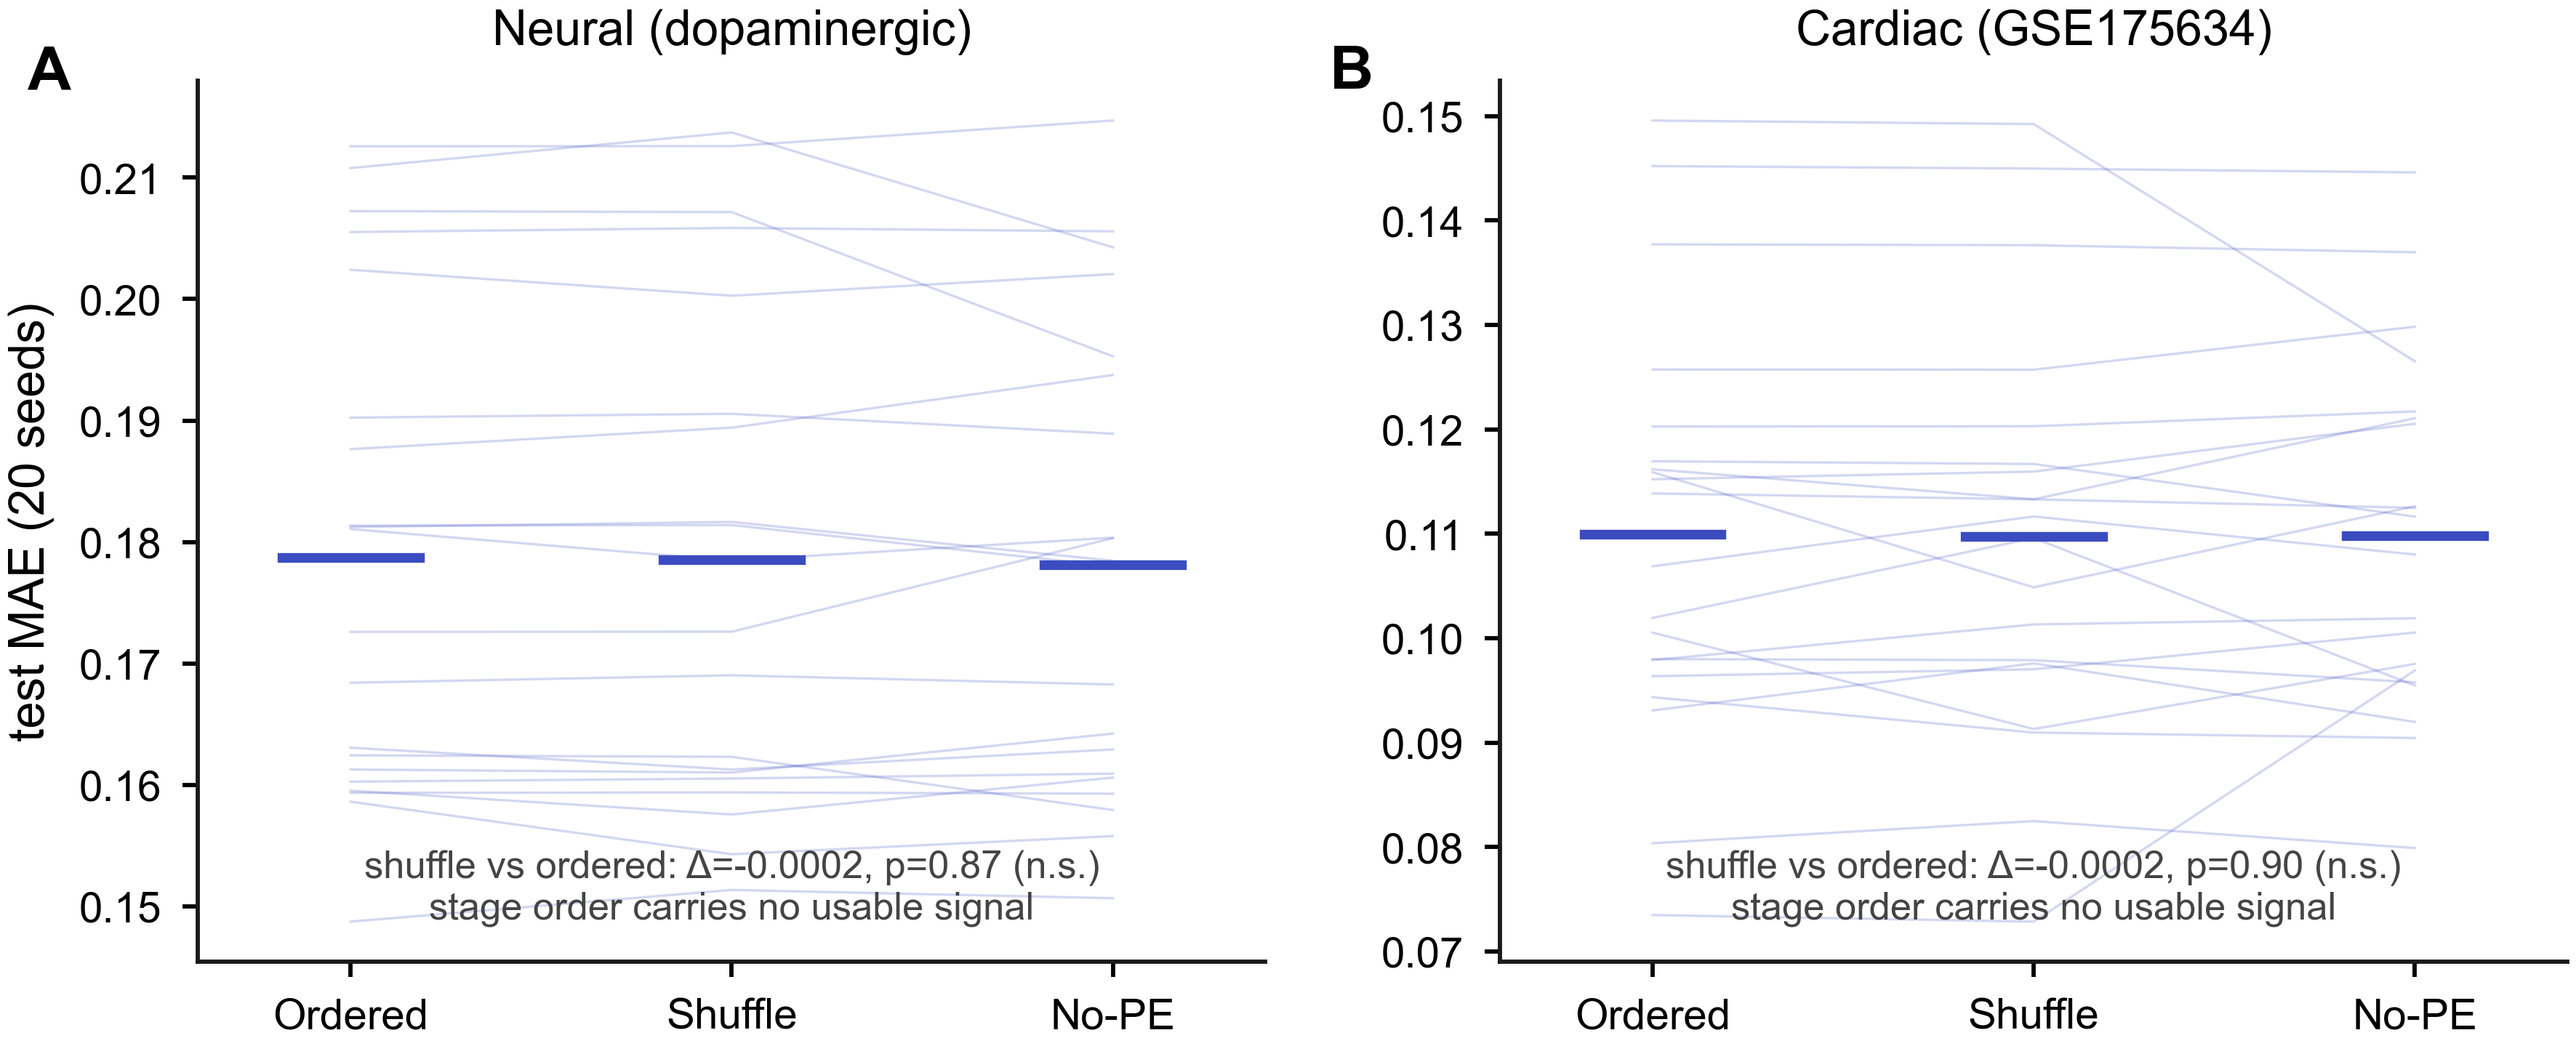
\includegraphics[width=0.92\textwidth]{figures/fig4_temporal.png}
\caption{\textbf{Destroying temporal order leaves accuracy unchanged.} Per-seed test MAE ($n=20$) for the Transformer under the ordered input, stage-order shuffle, and positional-encoding removal (no-PE) on the neural \textbf{(A)} and cardiac \textbf{(B)} lineages; faint lines are individual seeds and the bold bar is the per-condition mean. Shuffle-vs-ordered paired differences are $\overline{\Delta}=-0.0002$ ($p=0.87$, neural) and $-0.0002$ ($p=0.90$, cardiac), of order $1$--$3\%$ of the seed-to-seed standard deviation. Accuracy does not depend on positional information or a consistent input order; as the positive control shows, this control alone cannot establish the absence of temporal dependence.}
\label{fig:temporal}
\end{figure*}

\subsection{Mechanistic ODE}
Under the three calibration regimes of Sec.~\ref{sup:models} (main text, Fig.~4), per-trajectory calibration grants the ODE the most freedom to fit each test trajectory's early step, but because the trajectories pair independent cells, that early step carries no information about the late state; the additional freedom fits noise and generalizes worse. This is a statement about population-level priors on pseudo-trajectory data, not a general verdict on mechanistic modeling.

\subsection{Representation-sensitivity sweep}
Across the $38$ state-construction variants (main text, Fig.~5), per-feature errors show the expected lineage-specific difficulty pattern---the differentiation score is harder to predict than the pluripotency score on the cardiac lineage, and the reverse on the neural lineage---but model identity does not affect either component.

\section{Leakage Case Study: Index Handling}
\label{sup:leakage}

The earlier study's pipeline~\cite{kanu2026transformer} illustrates a general reproducibility failure: a model can appear superior when different predictors are evaluated on inconsistent trajectory indices. The Transformer was trained on a permuted partition of the $N=200$ trajectories but evaluated on a contiguous tail slice of the trajectory array that ignored the permutation, whereas the classical baselines were trained and scored on consistent, permuted partitions. Because the permuted training set draws roughly $70\%$ of all trajectory indices, the contiguous ``test'' slice overlaps heavily with training: $22$ of $30$ nominal test trajectories had been seen during training (Fig.~\ref{fig:leakage}). The Transformer was therefore evaluated largely on its own training data while the baselines were not, producing a \emph{relative} advantage that survives a casual comparison with baselines. Re-scoring every model on the identical frozen trajectories under one consistent split removes the advantage (main text, Table~3). The corrected protocol permutes indices once per seed and uses the resulting disjoint index sets identically for every model; \texttt{fair\_comparison.py} reproduces both evaluations from the frozen trajectories. This case study shows why benchmark implementations should make index membership explicit and apply identical splits to every model.

\begin{figure*}[!t]
\centering
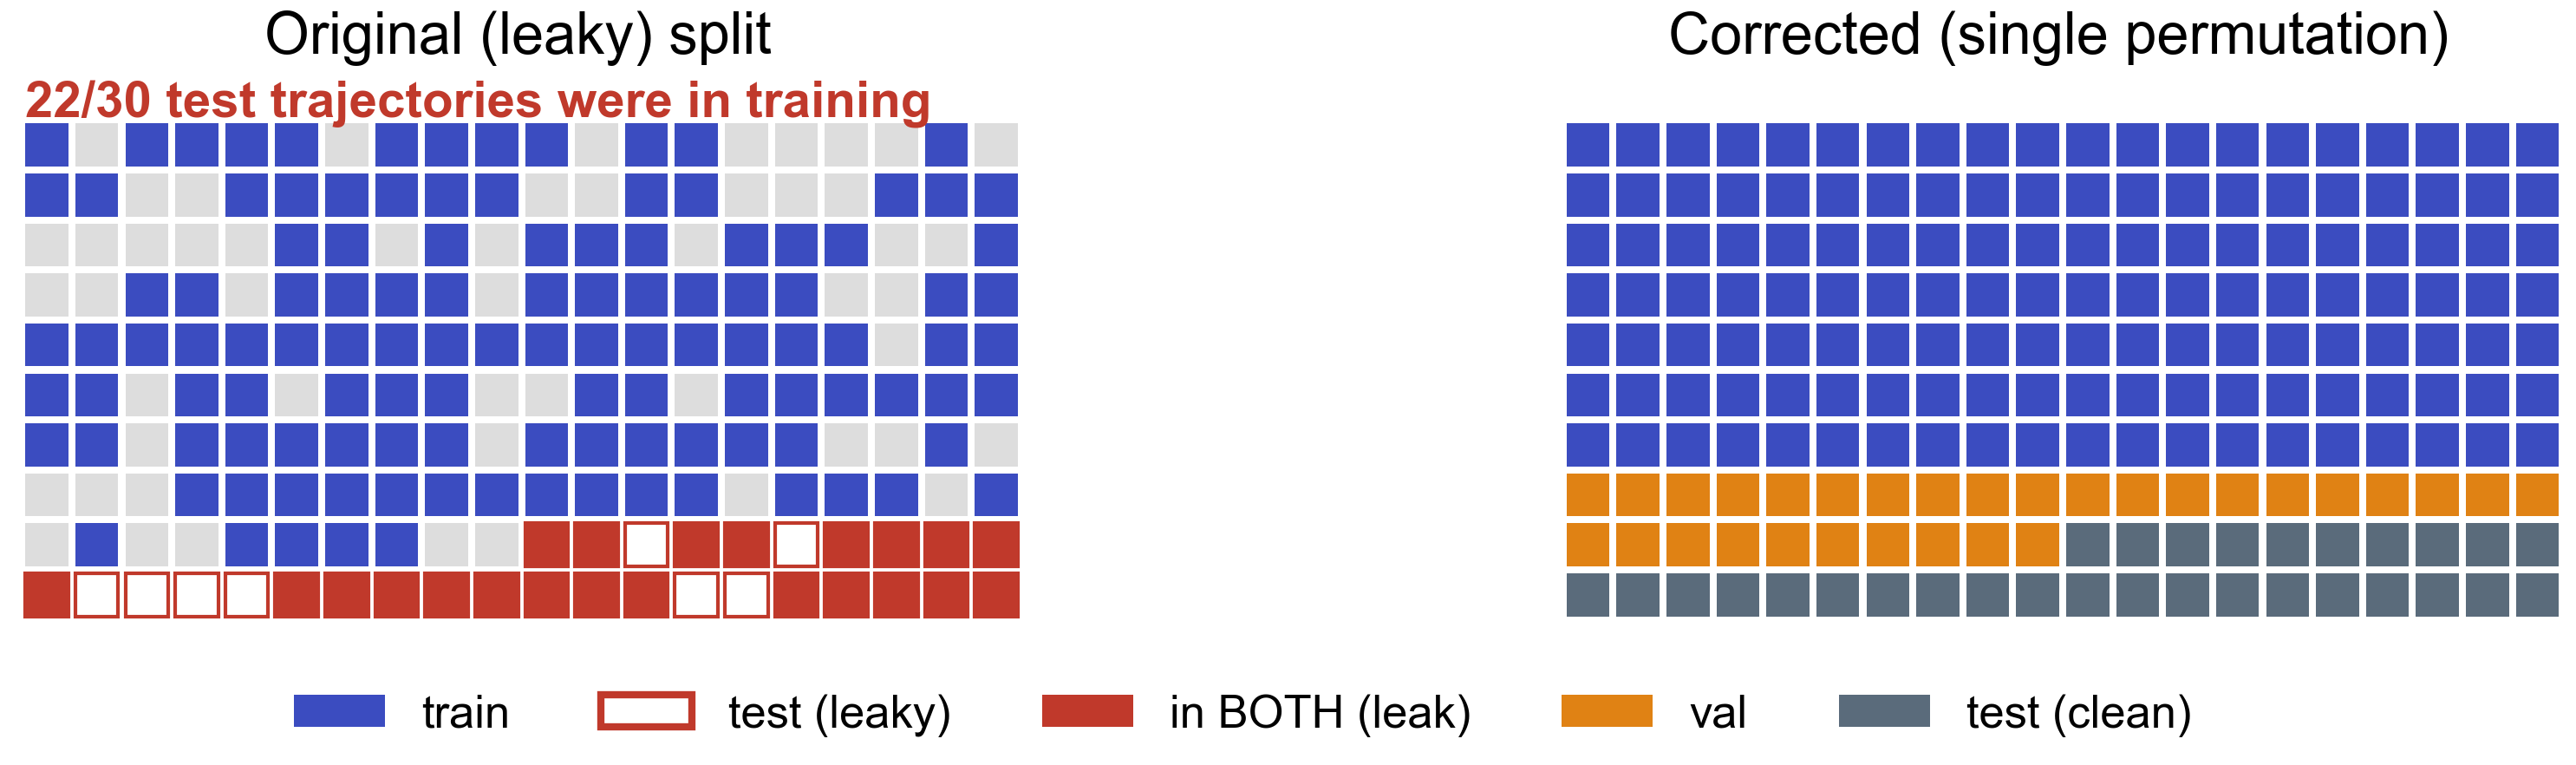
\includegraphics[width=0.92\textwidth]{figures/fig1_leakage_panel.png}
\caption{\textbf{The reported advantage originates in train--test leakage.} Trajectory-index membership for the $n=200$ pseudo-trajectories under the original (left) and corrected (right) splits. \emph{Left:} the model is trained on a permuted partition (blue) but evaluated on a contiguous tail slice (test, leaky); because the permuted training set spans $\sim$70\% of indices, $22$ of $30$ nominal test trajectories also appear in training (``in BOTH'', red). \emph{Right:} a single permutation yields disjoint train/validation/test blocks with no overlap. Only the Transformer was affected by the original asymmetry; all baselines were scored leakage-free.}
\label{fig:leakage}
\end{figure*}

\section{Implementation and Reproducibility}
\label{sup:impl}

All preprocessing and trajectory construction are seeded and serialized; every model consumes the same per-seed trajectories and split. Every figure and table value is generated programmatically from the per-seed JSON outputs; no reported number is entered by hand. Table~\ref{tab:impl_repro} summarizes the implementation stack. The code is available at \url{https://github.com/xaviwho/leakage-safe-benchmark} (MIT license; platform independent; dependencies pinned in \texttt{requirements.txt}, including PyYAML 6.0.3).

\begin{table*}[!t]
\centering
\caption{Implementation stack and reproducibility controls.}
\label{tab:impl_repro}
\footnotesize
\setlength{\tabcolsep}{4pt}
\begin{tabular}{>{\raggedright\arraybackslash}p{0.30\textwidth} >{\raggedright\arraybackslash}p{0.64\textwidth}}
\toprule
\textbf{Component} & \textbf{Specification} \\
\midrule
Environment A (original analyses: multi-seed comparisons, temporal controls, ODE calibration, representation sweep, leakage case study) & Python 3.14; package versions as recorded in the repository's \texttt{requirements.txt}: NumPy 2.4.3, SciPy 1.17.1, pandas 2.3.3, PyTorch 2.11.0 (CPU), scikit-learn 1.8.0, Scanpy 1.12.1, anndata 0.12.11, h5py 3.16.0, Matplotlib 3.10.8 \\
Environment B (revision analyses: constant baselines, positive controls, figures) & Python 3.12.10; NumPy 2.4.3, SciPy 1.17.1, pandas 2.3.3, PyTorch 2.11.0+cpu, scikit-learn 1.8.0, Scanpy 1.12.1, anndata 0.12.11, h5py 3.16.0, Matplotlib 3.10.8, POT 0.9.7.post1 \\
Cross-environment check & Ridge refitted in environment B on the regenerated per-seed data reproduces every stored per-seed MAE from environment A to within $10^{-16}$ on both lineages \\
ODE solver & \texttt{scipy.integrate.solve\_ivp} (RK45) \\
Calibration & Differential evolution (population-mean / distributional / per-trajectory) \\
Seeds & 20 seeds (10 for the $N=2{,}000$ positive controls); each perturbs trajectory construction \emph{and} model training \\
Statistics & Paired-bootstrap CI ($10^4$); Wilcoxon signed-rank; Cohen's $d_z$; Holm--Bonferroni \\
Datasets & Neural~\cite{jerber2021population}; cardiac \texttt{GSE175634}~\cite{elorbany2022single} \\
Normalization & Training-bounds min--max; clip to $[0,1]$ \\
Artifacts & Per-seed JSON metrics; every reported number generated by script from \texttt{results/} \\
\bottomrule
\end{tabular}
\end{table*}

\bibliographystyle{IEEEtran}
\bibliography{sn-bibliography}

\end{document}
